\documentclass{article}
\usepackage{graphicx} % Required for inserting images
\usepackage{subcaption}
%\usepackage[authordate,backend=biber]{biblatex-chicago}
\usepackage{natbib}

\title{Tweaking SSINS parameters for optimal outputs}
\author{Ridhima Nunhokee}
\date{}

\begin{document}

\maketitle

\section{Introduction}

Detection of the cosmological 21 cm hydrogen signal from the Epoch of Reionisation (EoR) remains one of the central goals of modern low-frequency radio astronomy. The expected brightness temperature fluctuations associated with the redshifted 21 cm line are extremely faint, typically on the order of approximately 10 mK, making detection highly susceptible to contamination from astrophysical foregrounds, instrumental systematics, and terrestrial Radio Frequency Interference (RFI).

Even weak contamination at amplitudes comparable to the cosmological signal can introduce systematic bias into power spectrum estimation, leading to false detections or incorrect interpretation of the underlying astrophysical processes \cite{Nunhokee2024, Kolopanis2019, Wilensky2019}. The challenge becomes particularly severe because current-generation interferometers do not directly image the cosmological signal, but instead rely on statistical measurements in Fourier space where residual contamination can mimic cosmological structure.

This work focuses on observations obtained using the Murchison Widefield Array (MWA) Phase III instrument. The upgraded correlator architecture was specifically introduced to mitigate known spectral artefacts associated with previous correlator implementations, where edge and central channels within each 3.24 MHz coarse frequency band required systematic flagging. These regularly missing channels produced harmonic structures in two-dimensional cylindrical power spectra, contaminating measurements within the EoR window.

Although hardware improvements reduce some systematic contamination, software-based RFI mitigation remains essential for ensuring robust cosmological analysis.

%One of the persistent challenges in decades of research in 21 cm cosmology is the presence of weak Radio Frequency Interference (RFI). Given that the expected amplitude of the 21 cm hydrogen signal is on the order of ~10 mK \citep{Furlanetto2016}, any interference of comparable or greater magnitude can significantly bias the results, leading to potential misinterpretation \cite{Nunhokee2024, Kolopanis2019, Wilensky2019}. It is therefore crucial to identify and mitigate such interference with great care.\\

%Current-generation instruments are limited to the statistical detection of the 21 cm hydrogen signal. This work presents observations from the third phase of the Murchison Widefield Array (MWA), which employs 128 antennas and an upgraded correlator. The new correlator was designed to alleviate bandpass filtering issues that previously required flagging of the edge and central channels within each 3.24 MHz coarse frequency band \citep{Tingay2013}. These gaps consequently introduced harmonic structures in the two-dimensional power spectra of the 21 cm hydrogen line.

\section{Problem Statement}

Current MWA preprocessing pipelines rely primarily on two automated flagging algorithms: AOFlagger and the Sky-Subtracted Incoherent Noise Spectra (SSINS) framework.

AOFlagger uses morphological and amplitude-based thresholding methods and performs well for strong RFI contamination \citep{Offringa2010}. However, previous work has demonstrated that default parameter settings can either fail to detect weak contamination or excessively remove clean data, particularly in low-SNR interferometric observations.

SSINS was introduced to improve statistical identification of contamination by analysing incoherent noise spectra after sky subtraction. While SSINS generally outperforms conventional threshold-based methods, practical analysis of MWA observations reveals inconsistent behaviour. Manual inspection shows three recurring problems:

\begin{itemize}
 \item Under-flagging, where weak contamination survives the detection stage (Figure~\ref{fig:under})
\item Over-flagging, where statistically normal fluctuations are incorrectly classified as interference (Figure~\ref{fig:over})
\item Observation-dependent variability, where a single parameter configuration performs inconsistently across different observations
\end{itemize}

The central challenge is therefore not simply tuning SSINS hyperparameters, but understanding whether the underlying statistical detection framework itself is sufficient for reliable RFI identification.

%Previous work with the MWA has relied on a combination of RFI flagging algorithms to mitigate contamination, most notably AOFlagger and the Sky-Subtracted Incoherent Noise Spectra (SSINS) method. AOFlagger has been found to produce undesirable results when run with its default settings \citep{Offringa2010}. While SSINS generally yields reasonable performance, manual inspection reveals that some observations suffer from under-flagging, whereas others are over-flagged. This work therefore focuses on identifying optimal paårameter settings that achieve a balanced trade-off between under- and over-flagging of data points.

%\begin{figure}[h]
%    \centering
%    \begin{subfigure}[b]{0.47\textwidth}
%        \centering
%        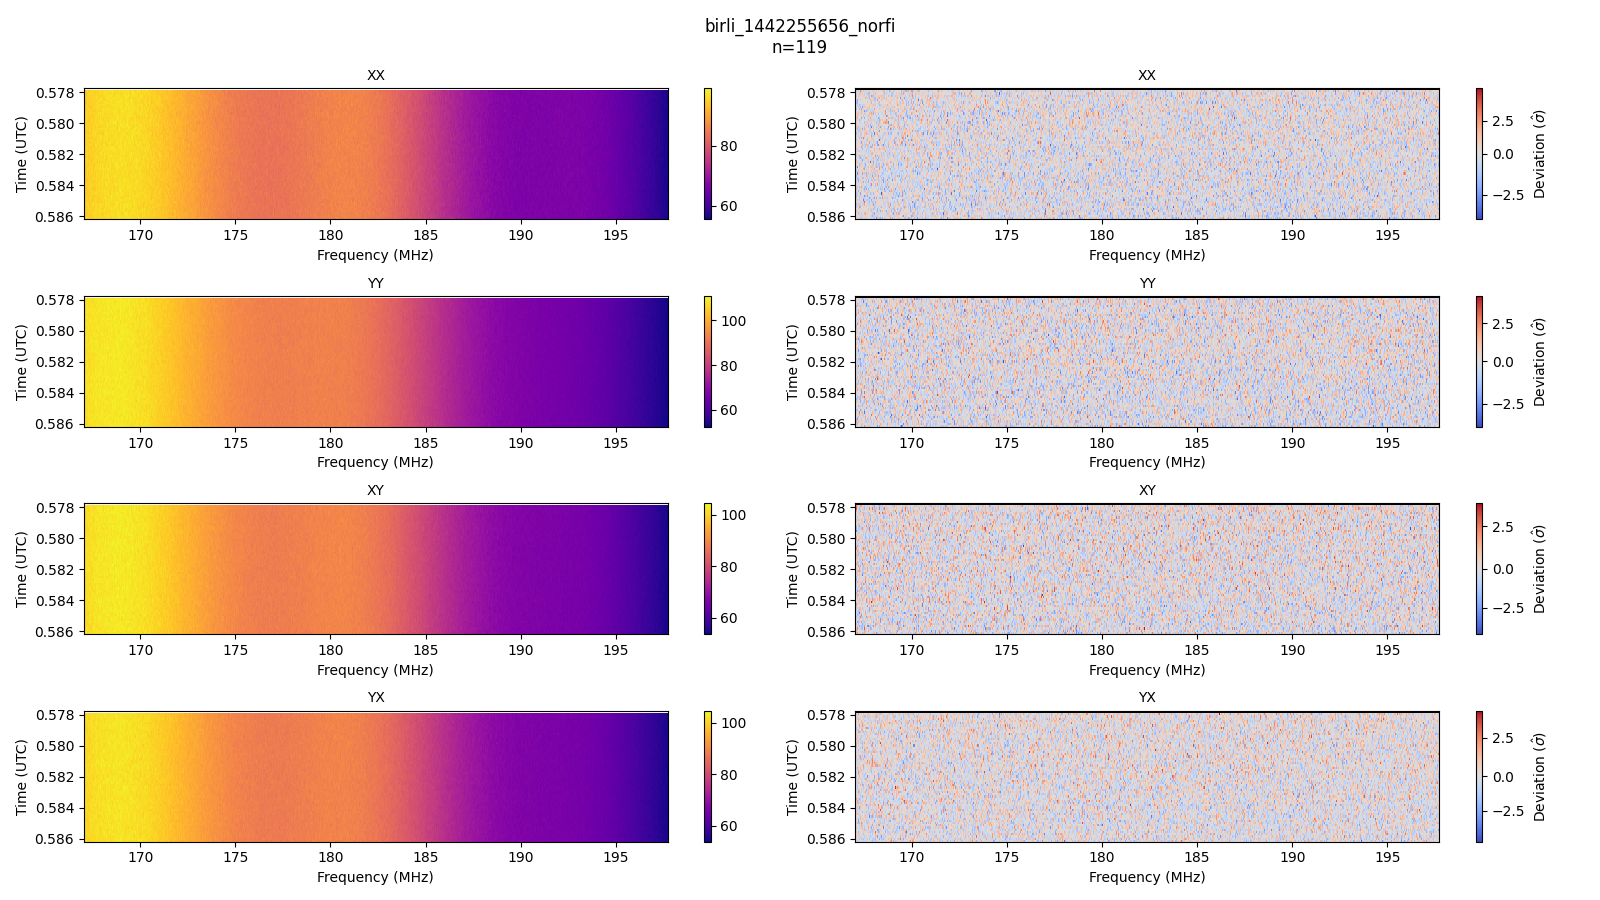
\includegraphics[width=\textwidth]{birli_1442255656_norfi_cross_SSINS.png}
%        \caption{Before SSINS flagging}
%        \label{fig:proper}
%    \end{subfigure}
%    \hfill
%    \begin{subfigure}[b]{0.47\textwidth}
%        \centering
%        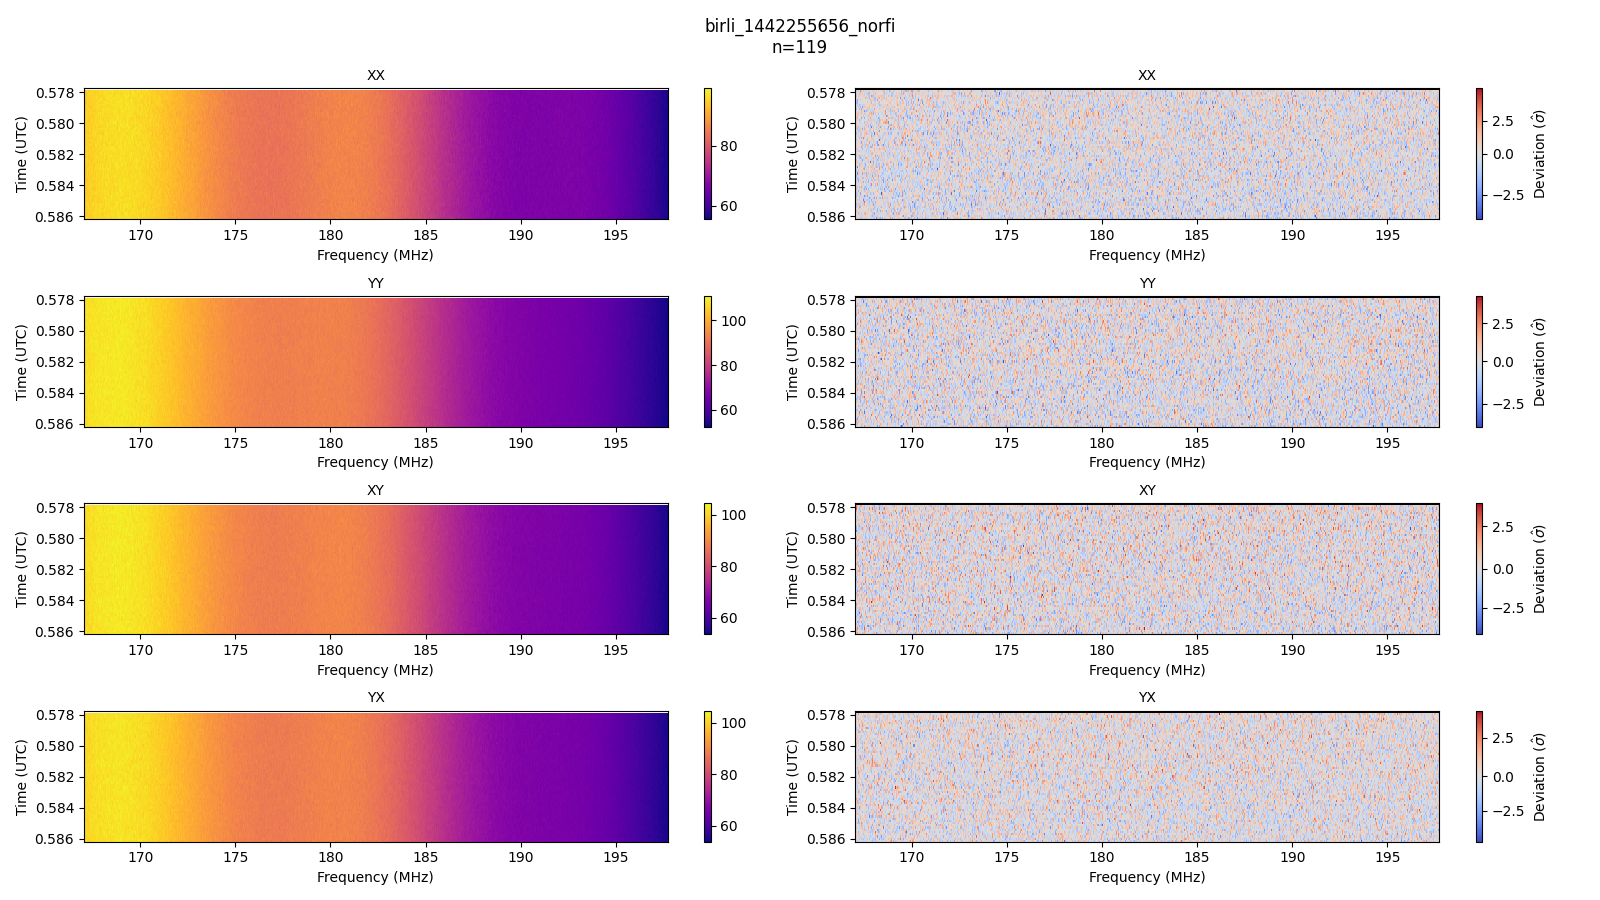
\includegraphics[width=\textwidth]{birli_1442255656_norfi_flagged_SSINS.png}
%        \caption{After SSINS flagging}
%        \label{fig:after}
%    \end{subfigure}
    
    %\caption{Comparison of visibilities before and after SSINS flagging for observation 1442255656.}
%\end{figure}

\begin{figure}[h]
    \centering
    \begin{subfigure}[b]{0.47\textwidth}
        \centering
        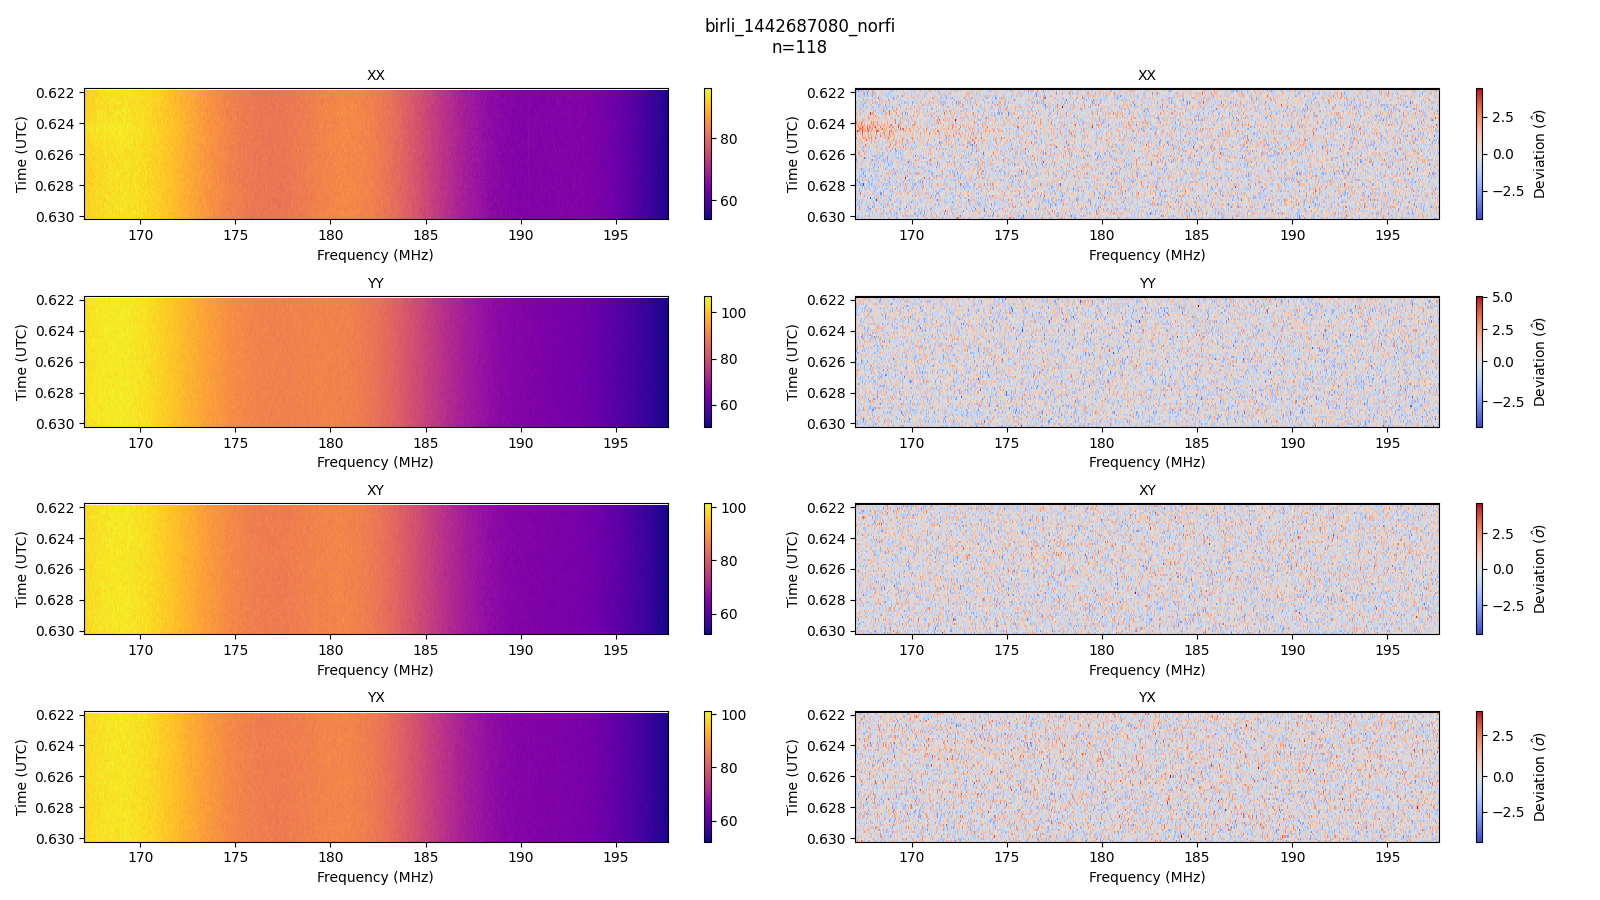
\includegraphics[width=\textwidth]{birli_1442687080_norfi_cross_SSINS.png}
        \caption{Before SSINS flagging}
        \label{fig:before}
    \end{subfigure}
    \hfill
    \begin{subfigure}[b]{0.47\textwidth}
        \centering
        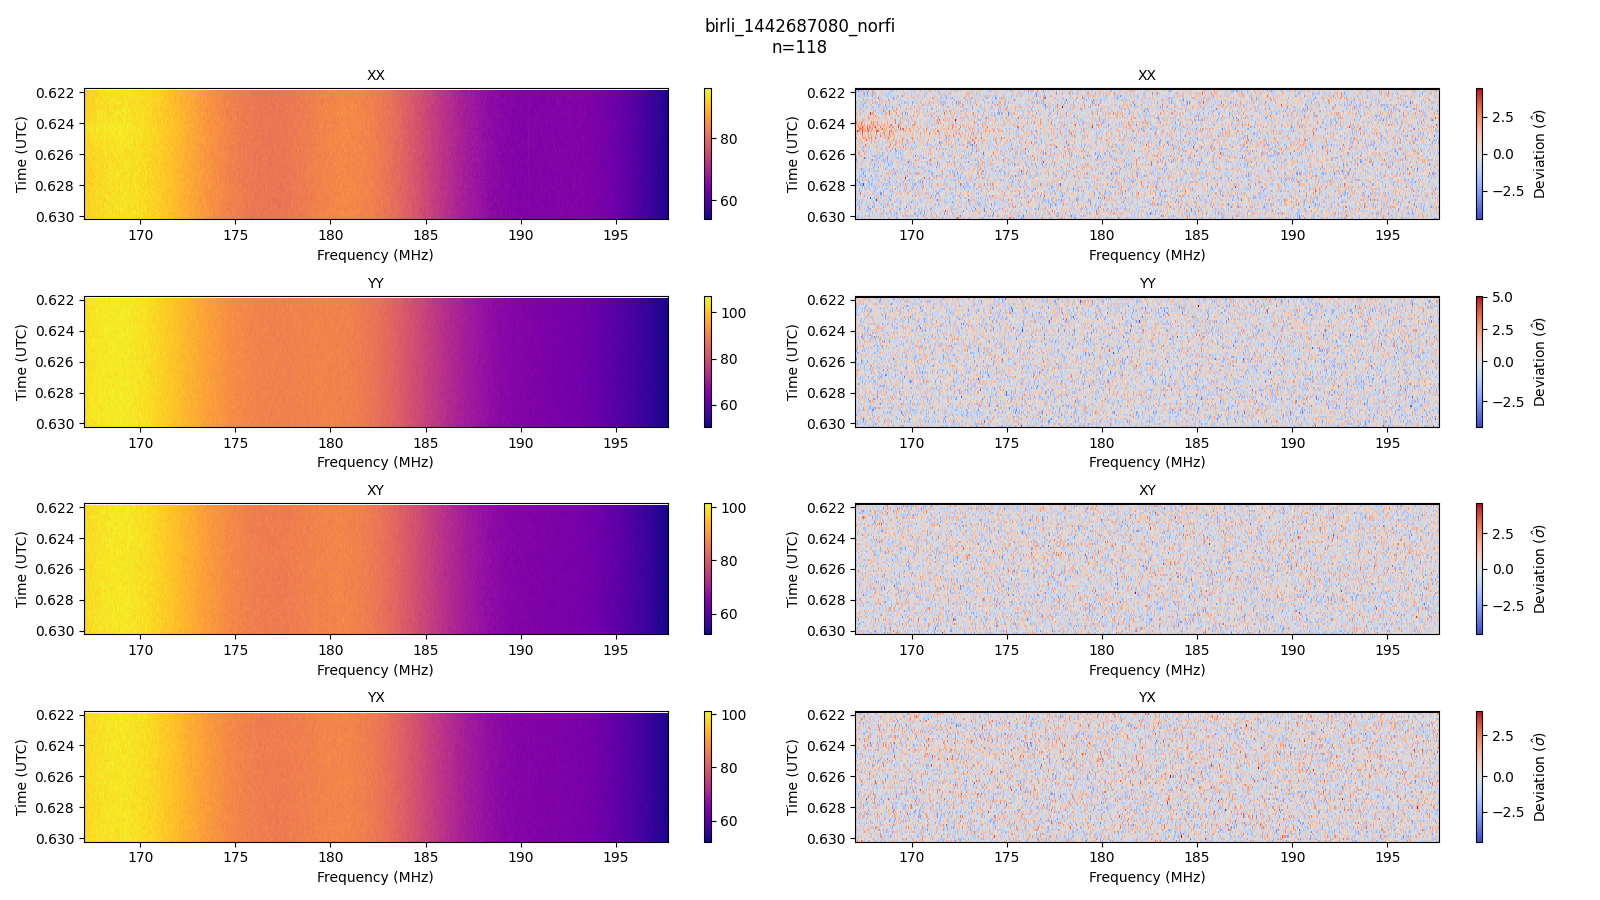
\includegraphics[width=\textwidth]{birli_1442687080_norfi_flagged_SSINS.png}
        \caption{After SSINS flagging}
        \label{fig:after}
    \end{subfigure}
    \caption{Comparison of visibilities before and after SSINS flagging for observation 1442687080.}
    \label{fig:under}
\end{figure}
\begin{figure}[h]
    \centering
    \begin{subfigure}[b]{0.47\textwidth}
        \centering
        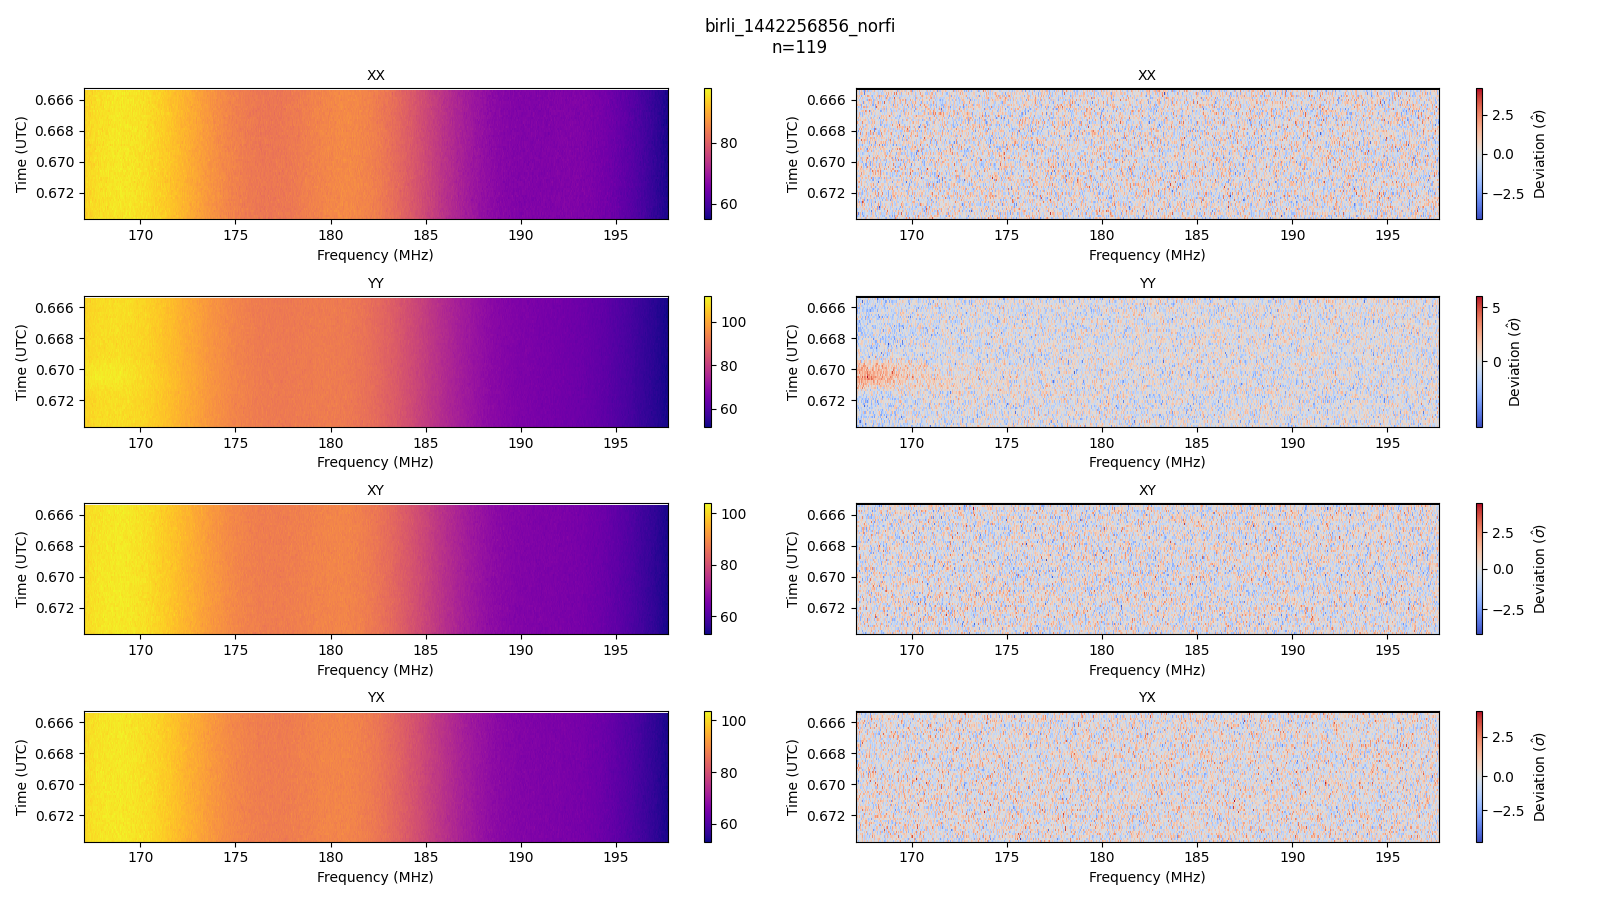
\includegraphics[width=\textwidth]{birli_1442256856_norfi_cross_SSINS.png}
        \caption{Before SSINS flagging}
        \label{fig:before}
    \end{subfigure}
    \hfill
    \begin{subfigure}[b]{0.47\textwidth}
        \centering
        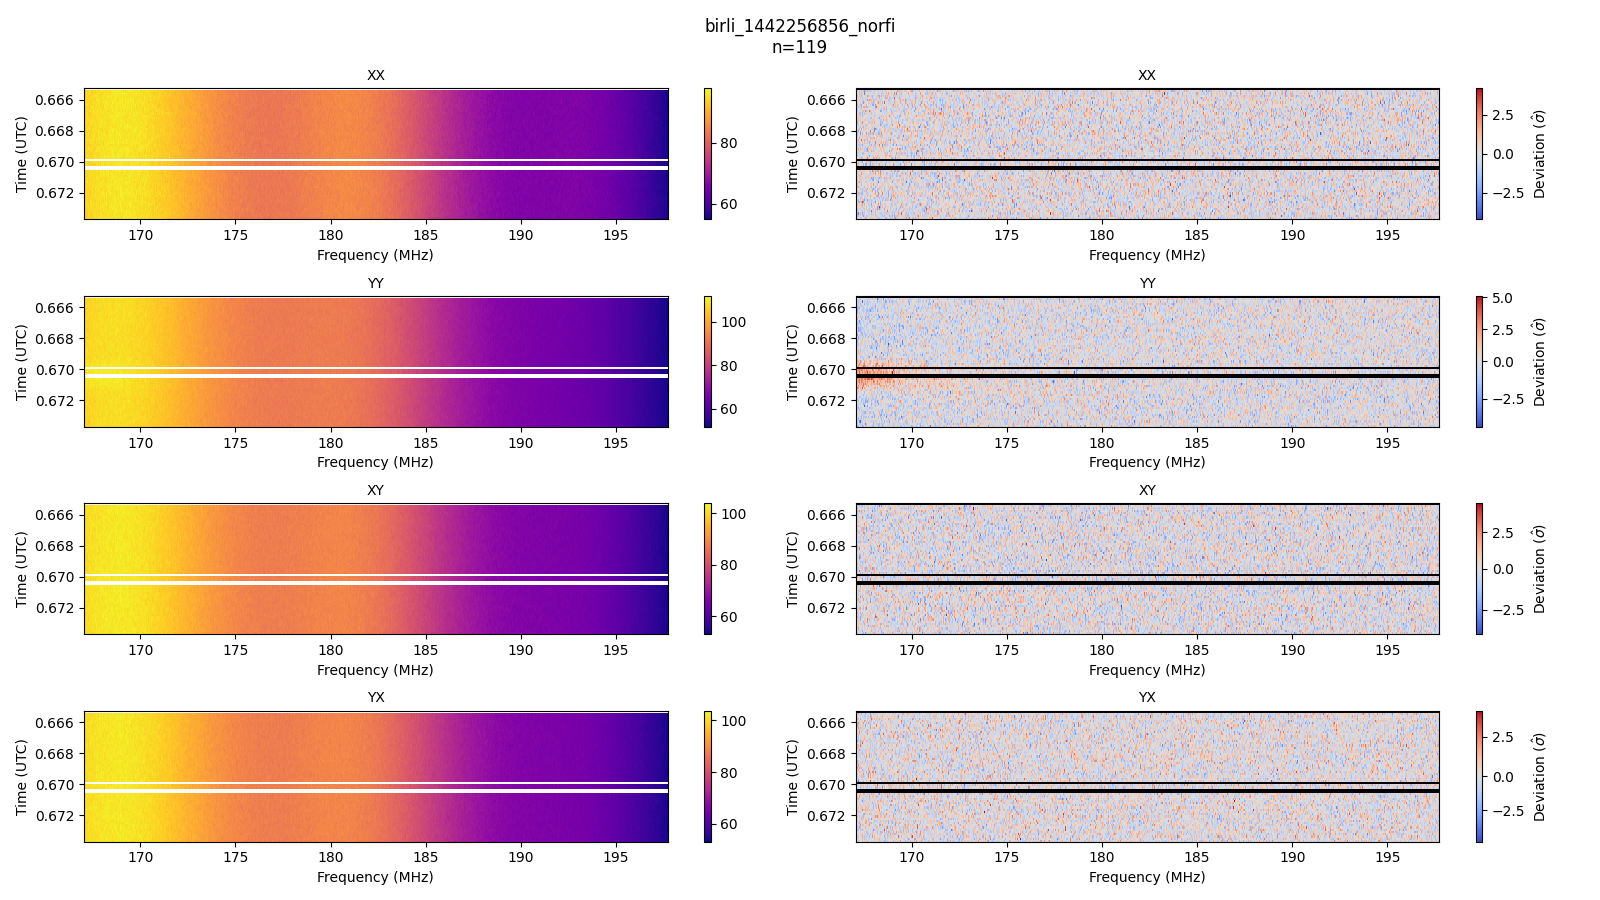
\includegraphics[width=\textwidth]{birli_1442256856_norfi_flagged_SSINS.png}
        \caption{After SSINS flagging}
        \label{fig:after}
    \end{subfigure}
    \caption{Comparison of visibilities before and after SSINS flagging for observation 1442256856.}
    \label{fig:over}
\end{figure}

\section{SSINS Statistical Framework}
SSINS detects anomalous visibility behaviour by constructing an incoherent noise spectrum from interferometric visibilities and evaluating deviations from expected thermal noise statistics. At its core, detection is based on the standard score (z-score):
\begin{equation}
z = \frac{x=\nu}{\sigma}
\end{equation}
where $x$ represents the observed visibility amplitude, $\nu$ is the expected mean thermal noise distribution and $\sigma$ represents the expected standard deviation. 

Large positive excursions indicate statistically anomalous behaviour that may correspond to RFI contamination. Unlike conventional amplitude thresholding methods, SSINS searches for deviations relative to the statistical noise model rather than absolute signal strength. This approach is particularly effective for identifying:
\begin{itemize}
\item Narrowband persistent transmitters
\item Broadband impulsive interference
\item Correlator artefacts
\item Cable reflections
\item Spectrally localised contamination structures
\end{itemize}
However, the statistical framework introduces several fundamental limitations.

\section{Why Z-Score Alone Is Not Sufficient for RFI Detection}
Although z-score statistics provide a mathematically convenient anomaly detection framework, they do not fully characterise the complexity of contamination present in radio interferometric observations. A large z-score does not necessarily imply RFI contamination, and conversely, contamination does not always produce large z-score excursions.Several limitations arise.

\subsection{Weak Persistent RFI May Not Produce Statistical Outliers}
SSINS assumes contamination manifests as statistical deviation from thermal noise behaviour. However, weak continuous interference may remain close to the underlying noise distribution.In such cases, $∣z∣<z_{thresh} $ despite contamination being physically present.

This leads to systematic false negatives, where weak interference propagates downstream undetected. This is particularly problematic in EoR experiments because weak contamination can accumulate coherently during long integration times and become visible only in power spectrum space.

\subsection{Instrumental Systematics Can Mimic Statistical Outliers}
Certain instrumental artefacts produce non-Gaussian deviations similar to RFI contamination such as cable reflections, gain calibration instabilities, correlator errors, bandpass ripple structures and cross-talk between antennas. These systematics can generate large $z$-score excursions despite not being true external RFI. This causes false positive detections, resulting in unnecessary data loss.

\subsection{Temporal Correlation Is Ignored}
The $z$-score framework evaluates each sample independently. However, many contamination sources exhibit temporal coherence, for example satellite passes, aircraft communication bursts and repeating transmission cycles. A single high z-score does not capture temporal evolution. Conversely, weak but temporally correlated contamination may remain statistically insignificant when evaluated independently.

\subsection{Spectral Morphology Is Ignored}
RFI sources exhibit characteristic spectral signatures.Examples include narrow carrier lines, frequency comb structures, harmonic periodicity
and broadband impulsive bursts. Two contamination events may produce identical $z$-score values while exhibiting completely different spectral behaviour. SSINS does not explicitly model spectral morphology.

\section{Hyperparameter Tuning Strategy}
The SSINS framework contains several sensitive hyperparameters controlling detection behaviour. The principal parameters investigated are:
\begin{enumerate}
\item Detection Threshold: Controls the z-score cutoff for anomaly detection.
\item Narrowband Detection Parameter: Controls sensitivity to spectrally localised contamination
\item Temporal-Spectral Aggregation: Controls smoothing across time-frequency structure.
\end{enumerate}
\section{Results}
Systematic parameter exploration reveals that no single hyperparameter configuration performs optimally across all observations.Three behavioural regimes emerge.

\subsection{Aggressive Flagging Regime}
For lower detection thresholds, typically below $4\sigma$, SSINS exhibits highly sensitive detection behaviour. In this regime, strong and moderate RFI structures are effectively removed; however, a substantial fraction of statistically consistent visibilities are incorrectly flagged. This over-flagging results in unnecessary loss of scientifically useful data and can negatively affect downstream calibration by reducing available visibility coverage. Observed characteristics include:
\begin{itemize}
\item High overall fraction of flagged data
\item Effective suppression of strong narrowband contamination
\item Increased false positive detections
\item Loss of astrophysical signal information
\end{itemize}
Although contamination removal is improved, the aggressive threshold introduces a clear trade-off between RFI suppression and signal preservation.

\subsection{Conservative Flagging Regime}
At higher threshold values, typically above $7\sigma$, SSINS becomes significantly less sensitive to contamination. In this regime, only the most statistically significant outliers are identified, resulting in lower overall flagging fractions and improved data retention.

However, visual inspection of post-flagging diagnostic plots reveals that weak contamination structures frequently remain undetected.This regime is characterised by:
\begin{itemize}
Lower fraction of flagged visibilities
\item Preservation of larger data volume
\item Weak persistent RFI remaining in the dataset
\item Residual contamination propagating into later pipeline stages
\end{itemize}
Although fewer false positives occur, undetected contamination can introduce systematic bias into subsequent power spectrum estimation.

\subsection{Intermediate Detection Regime}
Threshold values near the baseline configuration of approximately $5\sigma$ provide the most balanced overall performance. In this regime, a significant fraction of contamination structures are successfully removed while maintaining acceptable data retention. Observed improvements include:
\begin{itemize}
\item Reduction in coherent contamination structures in time-frequency space
\item Improved stability during calibration
\item Smoother downstream power spectrum behaviour
\item Reduced excessive loss of clean visibility data
\end{itemize}
However, despite improved performance relative to both aggressive and conservative parameter regimes, residual contamination structures remain visible in several observations.

\section{Observation-Dependent Variability}
A key result of this study is that identical SSINS parameter configurations behave inconsistently across different observations. Some observations required more aggressive thresholding to suppress strong contamination, while others exhibited excessive flagging under the same configuration. This variability indicates that contamination characteristics are strongly observation-dependent and that static parameter selection cannot reliably generalise across an entire dataset.

Representative analysis of multiple observations showed:
\begin{itemize}
\item Certain observations remained under-flagged despite moderate threshold values
\item Other observations experienced significant over-flagging under identical conditions
\item No globally optimal parameter configuration was identified across all tested observations
\end{itemize}
This demonstrates that fixed hyperparameter selection is fundamentally limited when applied to heterogeneous observational datasets.

\section{Limitations of $z$-Score-Based Detection}
An important result emerging from this analysis is that optimisation of SSINS hyperparameters alone cannot fully address contamination detection challenges.

Even under near-optimal threshold configurations, several contamination structures persist in the data without producing statistically significant $z$-score excursions. Conversely, instrumental systematics occasionally produce strong statistical deviations that are incorrectly classified as RFI contamination.

These findings suggest that z-score based anomaly detection is inherently limited because it assumes contamination is directly correlated with statistical deviation from expected thermal noise behaviour. However:
\begin{itemize}
\item Weak persistent RFI may remain statistically indistinguishable from background noise
\item Instrumental artefacts can generate false positive detections
\item Temporal and spectral coherence of contamination are not explicitly modelled
\end{itemize}
As a result, statistical threshold optimisation alone cannot guarantee robust contamination mitigation.

\section{Evaluation Metrics}
Performance of SSINS tuning is assessed using the following criteria:
\begin{itemize}
\item Flagging Fraction Stability: Ensuring consistent data retention across observations.
\item Residual RFI Suppression: Visual and statistical reduction of structured contaminants in z-score space.
\item Signal Preservation: Minimal distortion of astrophysical visibilities.
\item Downstream Impact: Improvement in calibration stability and power spectrum smoothness.
\end{itemize}
Evaluation should move beyond simply measuring fraction of flagged data. Recommended metrics include Statistical Metrics, Percentage flagged fraction, false positive rate, false negative rate, spectral Metrics, residual coherent spectral structure, bandpass smoothness, cosmological Metrics, improvement in EoR window cleanliness, reduction of wedge contamination, pipeline Metrics, calibration convergence stability and reduction in harmonic artefacts in power spectrum.

\section{Implications for Future RFI Mitigation}
The results demonstrate that while SSINS remains an effective first-stage statistical detection tool, reliance solely on z-score thresholding is insufficient for reliable identification of weak or structurally complex contamination.

The findings suggest that future RFI mitigation strategies should move beyond static threshold-based detection and incorporate additional diagnostic approaches such as:
\begin{itemize}
\item Adaptive observation-specific threshold selection
\item Morphological analysis of time-frequency contamination structures
\item Machine learning based anomaly detection frameworks
\item Downstream power spectrum feedback mechanisms for iterative re-flagging
\end{itemize}
These approaches may provide improved discrimination between true RFI contamination and instrumental systematics while preserving scientifically useful signal.
%\section{Beyond SSINS: What Should Be Done Next}

%\section{Conclusion}
%This work demonstrates that while SSINS provides an effective statistical framework for identifying strong contamination within MWA observations, its reliance on z-score statistics fundamentally limits its ability to identify weak persistent interference and distinguish true RFI from instrumental systematics.

%Hyperparameter tuning improves performance but cannot fully overcome these intrinsic limitations.The results suggest that future RFI mitigation strategies must move beyond purely statistical thresholding approaches toward hybrid frameworks incorporating temporal coherence, spectral morphology analysis, machine learning-based anomaly detection, and downstream power spectrum feedback.

%For next-generation EoR experiments, robust contamination mitigation will likely require adaptive intelligent pipelines rather than static threshold-based flagging algorithms.

%Only through such approaches can the extremely faint cosmological 21 cm signal be reliably separated from increasingly complex contamination environments.

%\section{SSINS Method and Role in the Pipeline}
%SSINS technique is designed to identify and mitigate systematic contamination in radio interferometric data by leveraging statistical deviations in visibility amplitude and phase structure. Unlike traditional flagging approaches that operate purely on amplitude thresholds, SSINS constructs a z-score statistic that quantifies deviations from expected thermal noise behaviour across time and frequency.

%In the context of MWA observations, SSINS is particularly effective at identifying both narrowband and broadband RFI, as well as instrumental systematics such as cable reflections and correlator artefacts. The output of SSINS is typically a mask or flagging solution that can be applied downstream in calibration and power spectrum estimation pipelines.

%However, the performance of SSINS is highly dependent on its hyperparameter configuration. Suboptimal parameter choices can either suppress genuine astrophysical signal (over-flagging) or allow residual RFI to propagate into subsequent analysis stages (under-flagging).


%\section{Hyperparameter Tuning Strategy}
%To address inconsistencies observed in previous runs, this work investigates systematic tuning of key SSINS parameters. The objective is to identify a parameter regime that maximises RFI suppression while preserving data volume and astrophysical signal integrity.

%\subsection{Threshold Selection}
%The primary tuning parameter is the z-score detection threshold. This parameter defines the statistical cutoff above which a data point is classified as contaminated. Low threshold values increase sensitivity but risk excessive flagging of noise fluctuations.
%High threshold values reduce false positives but may leave residual RFI structures unflagged. A practical tuning range is typically between 3 and 8, with initial runs centred around a threshold of 5 as a baseline reference.

%\subsection{Narrowband Sensitivity Control}
%The narrowband parameter determines the algorithm’s sensitivity to spectrally confined RFI features. This is particularly relevant for persistent carriers, satellite transmissions, and instrumentally induced spectral lines.
%Lower values improve detection of sharp spectral features.Higher values prioritise smoother spectral structure, reducing false detections. Given the variability of the RFI environment, this parameter should be tuned empirically using diagnostic z-score waterfall plots.

%\subsection{Temporal and Spectral Smoothing}
%SSINS performance is also influenced by smoothing scales applied in both time and frequency domains. These parameters control the trade-off between sensitivity to transient RFI and robustness against thermal noise fluctuations.
%Excessive smoothing may obscure short-duration RFI events. Insufficient smoothing may lead to noisy false positives. Optimal values depend on integration time and channel resolution of the dataset.

\section{Iterative Optimisation Procedure}
An iterative tuning framework is adopted to systematically refine SSINS performance:
\begin{enumerate}
\item Initial Run: Execute SSINS using baseline parameters (threshold $\approx$ 5).
\item Diagnostic Evaluation: Inspect z-score waterfall plots and flag distributions.
\item Adjustment Step:
Increase threshold if over-flagging is observed.
Decrease threshold if residual RFI structures persist.
\item Re-evaluation: Quantify improvements using
fraction of flagged data
reduction in coherent residual structure  and stability of downstream power spectra
\item Convergence Check: Iteration continues until additional parameter changes yield negligible improvement.
\end{enumerate}

%\section{Evaluation Metrics}

%\section{Considerations and Limitations}
%Several practical challenges arise during SSINS tuning:

%\begin{itemize}
%\item Sensitivity to dataset-specific RFI environments may require per-observation tuning.
%\item Multi-phase-center datasets may not be fully supported in certain SSINS implementations, leading to runtime errors or inconsistent outputs.
%\item Over-reliance on aggressive flagging can introduce bias in power spectrum estimation.
%\item Computational cost increases with iterative or grid-search-based tuning approaches.
%\end{itemize}

%\section{Conclusion}
%The effectiveness of SSINS in mitigating RFI within MWA observations is strongly dependent on careful hyperparameter selection. This work highlights the necessity of a structured, iterative tuning approach rather than reliance on default parameter settings. By systematically adjusting thresholding, narrowband sensitivity, and smoothing parameters, it is possible to achieve an optimal balance between RFI suppression and astrophysical signal preservation.

%Future work will focus on automating this tuning process through objective optimisation frameworks and integrating diagnostic feedback directly into the pipeline to enable adaptive, data-driven parameter selection.

\bibliographystyle{apalike}
\bibliography{references}

\end{document}
